%%\documentclass{beamer}
%%\documentclass[handout,usenames,dvipsnames]{beamer}
\documentclass[usenames,dvipsnames]{beamer}
\usepackage[numbers,totalnumber,sidebarshades]{beamerthemeUppsala}

\usepackage[utf8]{inputenc}
\usepackage[T1]{fontenc}
\usepackage{xcolor}
\usepackage{import}
\usepackage{listings}
\usepackage{hyperref}

%%%%%% Bibliograpy as footnotes %%%%
\usepackage{graphicx}
\usepackage[giveninits=true]{biblatex}
%\bibliography{../1DL010-21}

\graphicspath{{imgs/}}

\usepackage{pgfpages}
%\setbeameroption{show notes on second screen}
\setbeamertemplate{note page}{\insertnote}

%%\setbeamercovered{transparent}

\usepackage{xspace}
\usepackage{stmaryrd}
\usepackage{comment}

\newcommand{\tc}{\textcolor}
\newcommand{\largeskip}{\vspace{1cm}}
\newcommand{\nat}{\ensuremath{\mathbb{N}}}
\newcommand{\ra}{\ensuremath{\rightarrow}}

\newcommand{\states}{\ensuremath{S}}
\newcommand{\sts}{\ensuremath{s}}
\newcommand{\inits}{\ensuremath{s_I}}
\newcommand{\isg}{\ensuremath{g}}
\newcommand{\actions}{\ensuremath{A}}
\newcommand{\actf}{\ensuremath{\mathsf{av}}}
\newcommand{\acta}{\ensuremath{a}}
\newcommand{\trf}{\ensuremath{\delta}}
\newcommand{\costf}{\ensuremath{c}}
\newcommand{\utilf}{\ensuremath{u}}

\newcommand{\players}{\ensuremath{P}}
\newcommand{\maxp}{\ensuremath{\text{\textsc{max}}}}
\newcommand{\minp}{\ensuremath{\text{\textsc{min}}}}

\newcommand{\pts}{\ensuremath{PTS}}
\newcommand{\gts}{\ensuremath{GTS}}

\newcommand{\bstates}{\ensuremath{Q}}
\newcommand{\stb}{\ensuremath{q}}
\newcommand{\isf}{\ensuremath{f}}

\newcommand{\set}[1]{\ensuremath{ \{ #1 \}}}
\newcommand{\ol}{\ensuremath{\overline}}

\newcommand{\turnf}{\ensuremath{t}}

%%\newcommand{\land}{\wedge}
%%\newcommand{\lor}{\wee}
\newcommand{\lra}{\leftrightarrow}
\newcommand{\propl}{\mathcal{L}_p}

\newcommand{\M}{\mathcal{M}}
\newcommand{\lang}{\mathcal{L}}
\newcommand{\sat}{\ensuremath{\mathsf{SAT}}\xspace}
\newcommand{\limp}{\ensuremath{\mathsf{LIMP}}\xspace}

\newcommand{\const}{\boldsymbol}
\newcommand{\terms}{\mathit{TM}}
\newcommand{\term}{t}
\newcommand{\atoms}{ATOM}
\newcommand{\forms}{FORM}
\newcommand{\fv}{FV}
\newcommand{\struct}{\mathcal{S}}
\newcommand{\dom}{\Delta}

\newcommand{\intf}{I}

\newcommand{\te}{\ensuremath{\bar{v}}}
\newcommand{\va}{\ensuremath{v}}

\newcommand{\quant}{\ensuremath{\mathcal{Q}}}

\newcommand{\reals}{\ensuremath{\mathbb{R}}}

\newcommand{\hsig}{\ensuremath{h_{sig}}}
\newcommand{\logl}{\ensuremath{L_{\ell \ell}}}

\newcommand{\vechsig}{\ensuremath{\bar{h}_{sig}}}


%%%%%%%%%%%% Fabio ML %%%%%%%%%%%%%%%%%%
\def\riga{\vskip 1\baselineskip \noindent}
\newcommand{\bi}{\begin{itemize}\setlength{\itemsep}{-0.1em}}
\newcommand{\ei}{\end{itemize}}
\newcommand{\be}{\begin{enumerate}}
\newcommand{\ee}{\end{enumerate}}
%%%%%%%%%%%%%%%%%%%%%%%%%%%%%%%%%%%



%%%%%%%%%%% FNN %%%%%%%%%%%%%%%%%%%%
\newcommand{\nnw}[2]{w^{(#1)}_{#2}}
\newcommand{\nnW}[1]{\pmb{W}^{(#1)}}
\newcommand{\nna}[2]{a^{(#1)}_{#2}}
\newcommand{\nnA}[1]{\pmb{a}^{(#1)}}
\newcommand{\nnz}[2]{z^{(#1)}_{#2}}
\newcommand{\nnZ}[1]{\pmb{z}^{(#1)}}
\newcommand{\nnh}{\pmb{h}}
\newcommand{\nndelta}[2]{\delta^{(#1)}_{#2}}
\newcommand{\nnDELTA}[2]{\Delta^{(#1)}_{#2}}
\newcommand{\nnDelta}[1]{\pmb{\delta}^{(#1)}}
\newcommand{\nnDDELTA}[1]{\pmb{\Delta}^{(#1)}}


%%%%%%%%%%%%%%%%%%%%%%%%%%%%%%%%%%






%%%%%%%%%%%%%%%%%%%%%%%%%%%%%%%%%%%%%%%%
\title{1DT109 - Accelerating systems with FPGAs}
\subtitle{How to improve learning}

\author[R.\ De Masellis]{Riccardo De Masellis}
\date[]{\today}
\institute[uu.se]{Uppsala University}

\begin{document}

\begin{frame}[plain]
  \titlepage
\end{frame}
%%%%%%%%%%%%%%%%%%%%%%%%%%%%%%%%%%%%%%%
\section{Recap}
\frame{
\setbeamercovered{transparent}
\tableofcontents[currentsection,
        currentsubsection,
        subsectionstyle=shaded]
}
%%%%%%%%%%%%%%%%%%%%%%%%%%%%%%%%%%%%%%%
\begin{frame}
  \frametitle{The basis}

Supervised learning:

\begin{itemize}
\item $\pmb{x}$ input vector;
\item $y(\pmb{x})$ unknown function we want to approximate;
\item $\sigma(\pmb{x}, \pmb{w})$ hypothesis function;
\item loss and cost function. 	
\end{itemize}


\end{frame}
%%%%%%%%%%%%%%%%%%%%%%%%%%%%%%%%%%%%%%%

\begin{frame}
\frametitle{What we have seen so far}

We used \tc{blue}{squared error loss} (SE) function:
\[ 
   L_{sel}(\pmb{x}, y, \sigma) = (y(\pmb{x}) - \sigma(\pmb{x}, \pmb{w}))^2 = (y(\pmb{x}) - \frac{1}{1 + e^{-(\pmb{w}^T \pmb{x})}})^2
  \]
  
  \largeskip \pause
  
  The \tc{blue}{cost function} is therefore:
  %%
  \[
  C(\pmb{w}) = \frac{1}{2n} \sum_{i=1}^n  L_{sel}(\pmb{x}, y, \sigma) = \frac{1}{2n} \sum_{i=1}^n (y(\pmb{x}_i) - \frac{1}{1 + e^{-(\pmb{w}^T \pmb{x}_i)}})^2
  \]
  
  where $n$ is the number of examples in the training set.

  \end{frame}

%%%%%%%%%%%%%%%%%%%%%%%%%%%%%%%%%%%%%
\begin{frame}
  \frametitle{Gradient descent}
  
$\pmb{w}^{new} := [-\varepsilon, +\varepsilon]$ ($\varepsilon$ close to zero, e.g., 0.05) \tc{red}{IMPORTANT!}
 
 \bigskip
   
 do $\{$
 
 \bigskip
 
 $\quad \pmb{w}^{old} := \pmb{w}^{new}$
 
 \bigskip
 %%
$\quad w_0^{new} := w_0^{old} - \tc{red}{\eta} \frac{\partial C}{\partial w_0} (\pmb{w}^{old})$
 
 
$\quad \ldots$
 
$\quad w_m^{new} := w_m^{old} - \tc{red}{\eta} \frac{\partial C}{\partial w_m}(\pmb{w}^{old})$

\bigskip
  
  $\}$ while ( $C(\pmb{w}^{new}) < C(\pmb{w}^{old})$ )

\end{frame}
%%%%%%%%%%%%%%%%%%%%%%%%%%%%%%%%%%%%%%%

%%%%%%%%%%%%%%%%%%%%%%%%%%%%%%%%%%%%%%%
\begin{frame}
  \frametitle{Making gradient descent (GD) faster}
  
  Specifically for (FF) neural networks:
\begin{itemize}
\item stochastic GD: batch size = 1;
  \item batch GD: batch = training set;
  \item mini-batch GD:  1 < batch size < training set size;
  \item epoch.
\end{itemize}

\vspace{1cm}

Number of feed-forward pass and backpropagation pass in the above (training set size = n)?

\end{frame}

%%%%%%%%%%%%%%%%%%%%%%%%%%%%%%%%%%%%%%%
\section{Cross entropy loss function}
\frame{
\setbeamercovered{transparent}
\tableofcontents[currentsection,
        currentsubsection,
        subsectionstyle=shaded]
}
%%%%%%%%%%%%%%%%%%%%%%%%%%%%%%%%%%%%%%%

 
 %%%%%%%%%%%%%%%%%%%%%%%%%%%%%%%%%%%%%%%

\begin{frame}
\frametitle{Problems with squared error loss}

EASY SETTING: \tc{blue}{one} neuron, binary classification, \tc{blue}{two} weights $w$ (including bias) and \tc{blue}{one} training example $x$.

\pause

\[ C(\pmb{w}) = \frac{\tc{blue}{1}}{2} (y(x) - \sigma(x, \pmb{w}))^2 \]

\begin{ntblock}
\[ \frac{\partial C}{\partial w_0} = (\sigma(x, \pmb{w}) - y(x)) \frac{\partial \sigma}{\partial \pmb{z}} x \]
\end{ntblock}

What happens when the neuron \tc{red}{badly misclassify}?

\pause

\begin{itemize}
  \item $| \sigma(x, \pmb{w}) - y(x) | \approx 1$ which means that:
  \item either \tc{blue}{$\sigma(x, \pmb{w}) = 0$} (and $y(x)=1$) or \tc{blue}{$\sigma(x, \pmb{w}) = 1$} (and $y(x)=0$) ...
 \end{itemize}

\end{frame}


%%%%%%%%%%%%%%%%%%%%%%%%%%%%%%%%%%%

\begin{frame}
  \frametitle{Problems with squared error loss: SLOW}
  
  \begin{center}
  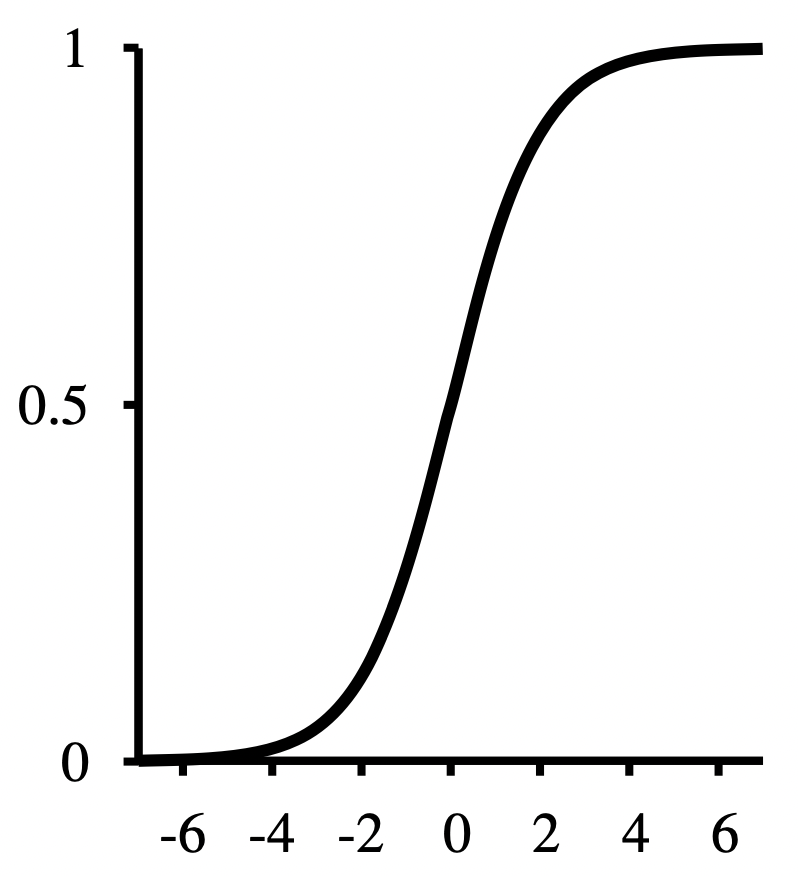
\includegraphics[scale=.2]{sigmoid}	
  \end{center}

When \tc{blue}{$\sigma(x, \pmb{w}) = 0$} or \tc{blue}{$\sigma(x, \pmb{w}) = 1$} then \tc{red}{$\frac{\partial C}{\partial w_0}(\pmb{w}) \approx 0$} therefore, recalling the update rule of GD: 
  
  \[\quad w_0^{new} := w_0^{old} - \eta \frac{\partial C}{\partial w_0} (w^{old})\] 
  
  \pause
 
\begin{alertblock}{}
\centering
The learning is \tc{red}{very slow} at the beginning!
\end{alertblock}

(The same intuition also applies to deep network.)

\end{frame}


%%%%%%%%%%%%%%%%%%%%%%%%%%%%%%%%%%%%%%%

\begin{frame}{Problems with squared error loss: NON-CONVEX}

  \[
  C(\pmb{w}) = \frac{1}{2n} \sum_{i=1}^n  L_{sel}(\pmb{x}, y, \sigma) = \frac{1}{2n} \sum_{i=1}^n (y(\pmb{x}_i) - \frac{1}{1 + e^{-(\pmb{w}^T \pmb{x}_i)}})^2
  \]
  
  \bigskip
  
  A function $C$ is \tc{red}{convex} if it is twice differentiable and its second derivative $\frac{\partial^2{C}}{{\partial \pmb{w}^2}}$ is positive for all $\pmb{w}$. A convex function has a global minimum.
  
  \bigskip
  
  \begin{alertblock}{}
\centering
C(\pmb{w}) is \tc{red}{NON-CONVEX} (in general): it might  have \tc{red}{local minima}!
\end{alertblock}
 
\end{frame}

%%%%%%%%%%%%%%%%%%%%%%%
%%%%%%%%%%%%%%%%%%%%%%%%%

%%%%%%%%%%%%%%%%%%%%%%%%%%%
\begin{frame}
  \frametitle{Introducing: cross-entropy loss function}
  
  
  \begin{definition}[Cross-entropy loss function]
  Let $\pmb{x}$ be an example, $y(\pmb{x})$ a target function and $\sigma(\pmb{x}, \pmb{w})$ an hypothesis:
  	\[
  	\crosse(\pmb{x}, y, a) = 
  	\begin{cases}
  		-log(\sigma(\pmb{x}, \pmb{w})) \quad \quad \; \; \text{ if } y(\pmb{x})=1 \\
  		-log(1 - \sigma(\pmb{x}, \pmb{w})) \quad \text{ if } y(\pmb{x})=0
  	\end{cases}
  	\]
  \end{definition}
  
  \medskip \pause

\begin{minipage}[c]{0.5\textwidth}
	\centering
	
	\[log(z)\]
	
	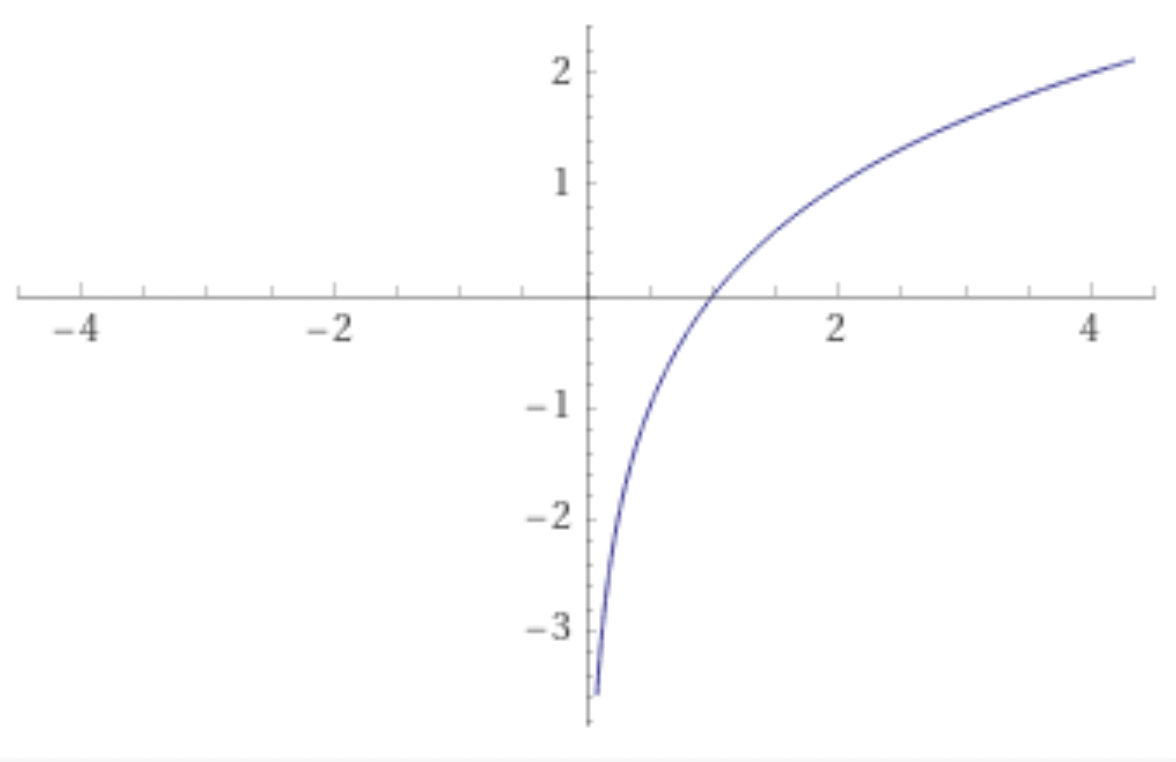
\includegraphics[scale=.25]{log2x}
\end{minipage}\begin{minipage}[c]{0.5\textwidth}
	\centering
	
	\[log(1-z)\]
	
	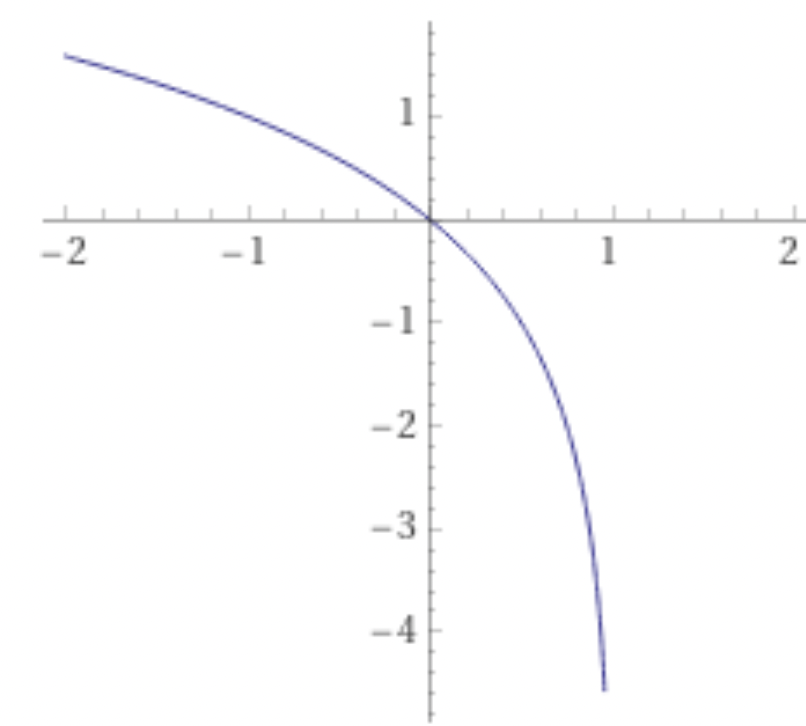
\includegraphics[scale=.25]{log2(1-x)}
\end{minipage}

\end{frame}
%%%%%%%%%%%%%%%%%%%%%%%%%%%

%%%%%%%%%%%%%%%%%%%%%%%%%%%
\begin{frame}
  \frametitle{Cross-entropy loss function}
  \[
  	\crosse(\pmb{x}, y, \sigma) = 
  	\begin{cases}
  		-log(\sigma(\pmb{x}, \pmb{w})) \quad \quad \; \; \text{ if } y(\pmb{x})=1 \\
  		-log(1 - \sigma(\pmb{x}, \pmb{w})) \quad \text{ if } y(\pmb{x})=0
  	\end{cases}
  	\]
  	
  	\[
  	\crosse(\pmb{x}, y, \sigma) = -y(\pmb{x}) \; log(\sigma(\pmb{x}, \pmb{w})) -(1-y(\pmb{x})) \; log(1 - \sigma(\pmb{x}, \pmb{w}))
  	\]


 %% \medskip
  
\begin{minipage}[c]{0.5\textwidth}
	\centering
	
	\[-log(z)\]
	
	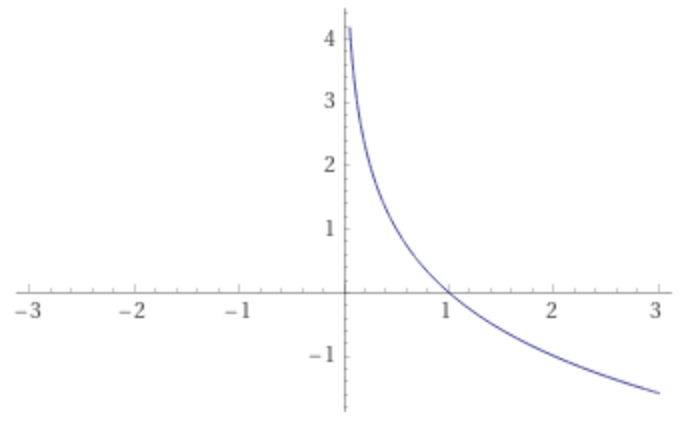
\includegraphics[scale=.4]{-log2x}
\end{minipage}\begin{minipage}[c]{0.5\textwidth}
	\centering
	
	\[-log(1-z)\]
	
	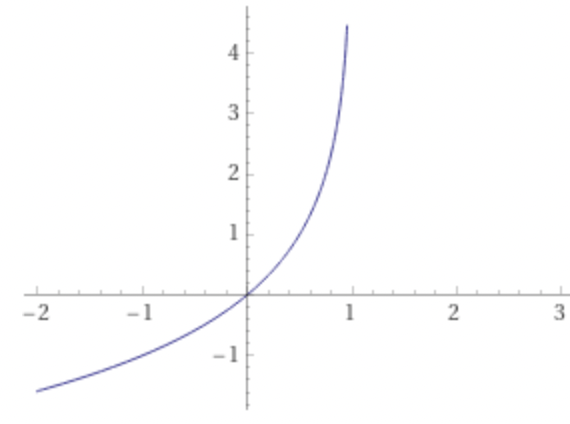
\includegraphics[scale=.4]{-log2(1-x)}
\end{minipage}

\end{frame}
%%%%%%%%%%%%%%%%%%%%%%%%%%%
\begin{frame}
  \frametitle{Good news}
  
  If we take $\crosse$ as loss function, then the cost function is:
  %%
  \[
  C(\pmb{w}) = \frac{1}{n} \sum_{i=1}^{n} \crosse(\pmb{x}_i, y, \sigma) = 
  \]
  %%
  \[ -\frac{1}{n} \sum_{i=1}^{n} (y(\pmb{x}_i) \; log(\sigma(\pmb{x}_i, \pmb{w})) + (1-y(\pmb{x}_i)) \; log(1 - \sigma(\pmb{x}_i, \pmb{w})))  \]
    
\end{frame}

%%%%%%%%%%%%%%%%%%%%%%%%%%%%%%%%%%%%%%%%

\begin{frame}
  \frametitle{Good news \#1}
  
  \[ C(\pmb{w}) = -\frac{1}{n} \sum_{i=1}^{n} (y(\pmb{x}_i) \; log(\sigma(\pmb{x}_i, \pmb{w})) + (1-y(\pmb{x}_i)) \; log(1 - \sigma(\pmb{x}_i, \pmb{w})))  \]
  
    \begin{alertblock}{}
   \centering
In a NN with no hidden layers, it is \tc{red}{convex} and it always has a \tc{red}{global minimum}, regardless of the TS (with hidden layers, it is not always the case).
  \end{alertblock}
  
  \end{frame}
%%%%%%%%%%%%%%%%%%%%%%%%%%%%%%%%%%%%%%%%

\begin{frame}
\frametitle{Good news \#2}

  \[ C(\pmb{w}) = -\frac{1}{M} \sum_{i=1}^{M} (y(\pmb{x}_i) \; log(\sigma(\pmb{x}_i, \pmb{w})) + (1-y(\pmb{x}_i)) \; log(1 - \sigma(\pmb{x}_i, \pmb{w})))  \]

Let's compute the partial derivative wrt $w_j$:

\[
\frac{\partial C}{\partial w_j} = \frac{1}{n} \sum_{i=1}^n \left( \frac{y(x)}{ \sigma(\pmb{x}_i, \pmb{w} ) } - \frac{1-y(\pmb{x}_i)}{1 - \sigma(\pmb{x}_i, \pmb{w})} \right) \frac{\partial \sigma}{\partial w_j}
\]

by doing some math we end up with:

\[
\frac{\partial C}{\partial w_j} = \frac{1}{n} \sum_{i=1}^n x_j(\sigma(\pmb{x}_i, \pmb{w}) - y(\pmb{x}_i))
\]

\pause

\begin{alertblock}{}
\centering
	\tc{red}{Now the update on weights depends on the error in the output $\sigma(\pmb{x}_i, \pmb{w}) - y(\pmb{x}_i)$!}
\end{alertblock}


 \end{frame}


%%%%%%%%%%%%%%%%%%%%%%%%%%%%%%%%%%%%%%%
%%%%%%%%%%%%%%%%%%%%%%%%%%%%%%%%%%%%%%%
\section{Overfitting}
\frame{
\setbeamercovered{transparent}
\tableofcontents[currentsection,
        currentsubsection,
        subsectionstyle=shaded]
}
%%%%%%%%%%%%%%%%%%%%%%%%%%%%%%%%%%%%%%%

\begin{frame}
	\frametitle{Overfitting}
	
	\begin{alertblock}{Problem}
		When do we stop the learning phase?
	\end{alertblock}
	
	\pause
	
	Recall: we have \tc{blue}{training} set and \tc{blue}{test} set. Clearly, the more we train, the less the cost $C_{train}$ (on the training set) becomes:

\begin{center}
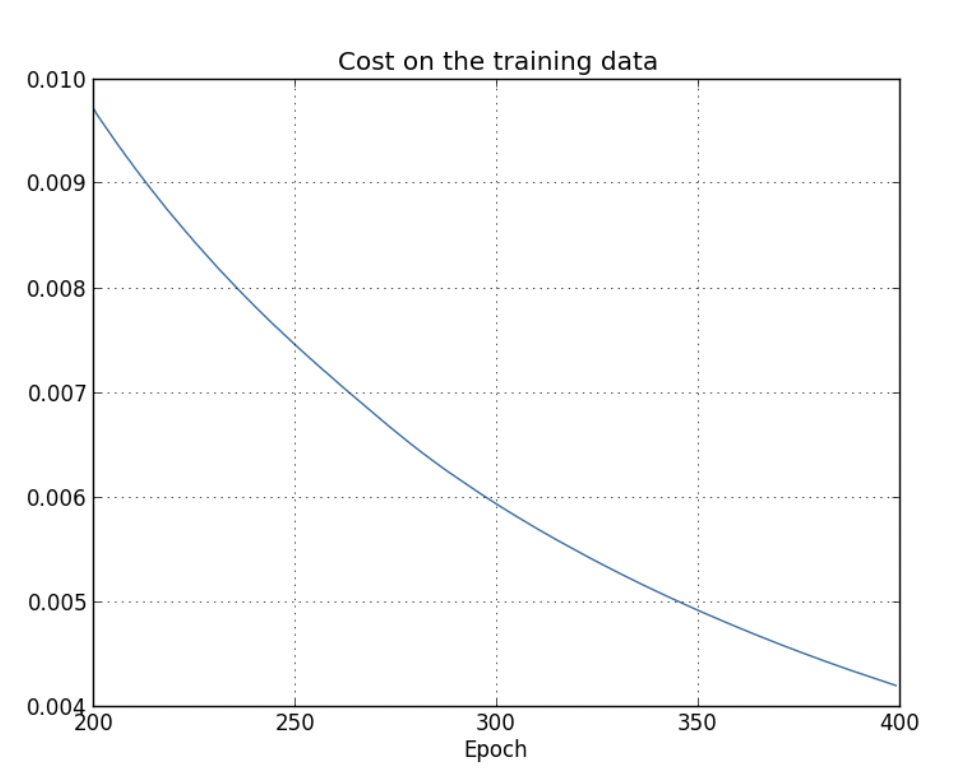
\includegraphics[scale=.3]{cost-train}
\end{center}

{\tiny 30 hidden neurons, a mini-batch size of 10, 400 epochs, 1000 training images, $\eta=0.5$.}
	
\end{frame}
%%%%%%%%%%%%%%%%%%%%%%%%%%%%%%%%%%%%%%%

\begin{frame}
\frametitle{Overfitting, cont'd}

But if we look at the classification accuracy on the \tc{blue}{test} set:

\begin{center}
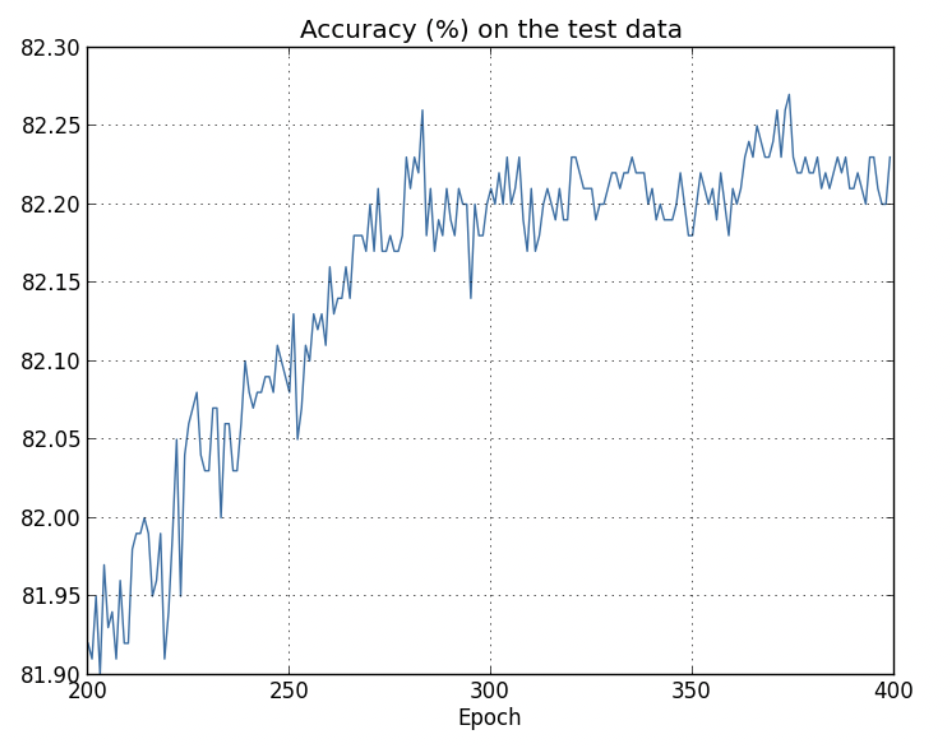
\includegraphics[scale=.3]{accuracy-test}
\end{center}

After around epoch 280, the model does not get better accuracy. It is \tc{red}{overfitting the training data}. That is: it is specialising in perfectly recognising the train examples, but it does not \tc{red}{generalise} on new examples.
	
\end{frame}



%%%%%%%%%%%%%%%%%%%%%%%%%%%%%%%%%%%%%%%
\begin{frame}
  \frametitle{The validation set}
  
  We can use another set, the \tc{blue}{validation} set, and we use this to compute the accuracy (instead of using the training set) for choosing hyper-parameters. We stop when the accuracy does not improve (\emph{early stopping} strategy).
  
  \medskip
  
  Why?
  
  \medskip \pause
  
  If we used the test set, we would overfit the hyper-parameters to the test set.
  
\end{frame}


%%%%%%%%%%%%%%%%%%%%%%%%%%%%%%%%%%%%%

\begin{frame}
  \frametitle{Always better to have lots of data}
  
  \begin{ntblock}
  	\centering
  	When you have a lot of data, overfitting is never a problem!
  \end{ntblock}
  
\end{frame}



%%%%%%%%%%%%%%%%%%%%%%%%%%%
\section{Regularization}
\frame{
\setbeamercovered{transparent}
\tableofcontents[currentsection,
        currentsubsection,
        subsectionstyle=shaded]
}

%%%%%%%%%%%%%%%%%%%%%%%%%%%%%%%%%%%%%%%

\begin{frame}
  \frametitle{Avoiding overfitting: regularization}
  
  \tc{red}{Weight decay} regularization:
  
\[ C(\pmb{w}) = -\frac{1}{n} \sum_{i=1}^{n} (y \; log(\sigma)) + (1-y) \; log(1 - \sigma) + \tc{red}{\frac{\lambda}{2n} \sum_{j=1}^{m} w_m^2} \]


\begin{alertblock}{Idea:}
\centering
	bias towards small weights.
\end{alertblock}
\end{frame}

%%%%%%%%%%%%%%%%%%%%%%%%%%%%%%%

\begin{frame}
  \frametitle{What happens with regularization term}
  
  \[ C(\pmb{w}) = C_0 + \tc{red}{\frac{\lambda}{2n} \sum_{j=1}^{m} w_m^2} \]
  
  
  The partial derivatives wrt $w$ (bias excluded) are:
  
\[
\frac{\partial C}{\partial w} = \frac{\partial C_0}{\partial w} + \frac{\lambda}{n}w
\]


The new gradient descent updates the weights in this way:


\[ w_{new} = w_{old} -\eta \frac{\partial C_0}{\partial w}(\pmb{w}_{old}) - \frac{\eta \lambda}{n} w_{old} = \tc{red}{(1 - \frac{\eta \lambda}{n})}w_{old} -\eta \frac{\partial C_0}{\partial w}(\pmb{w}_{old}) \]

  notice the \tc{red}{weight decay}, making the weight smaller.
  
\end{frame}

%%%%%%%%%%%%%%%%%%%

\begin{frame}
  \frametitle{Does it work? ($\lambda = 0.1$, TS size = 1000)}
  
  \begin{minipage}{.4\textwidth}
  \begin{center}
  {\tiny With regularization}
  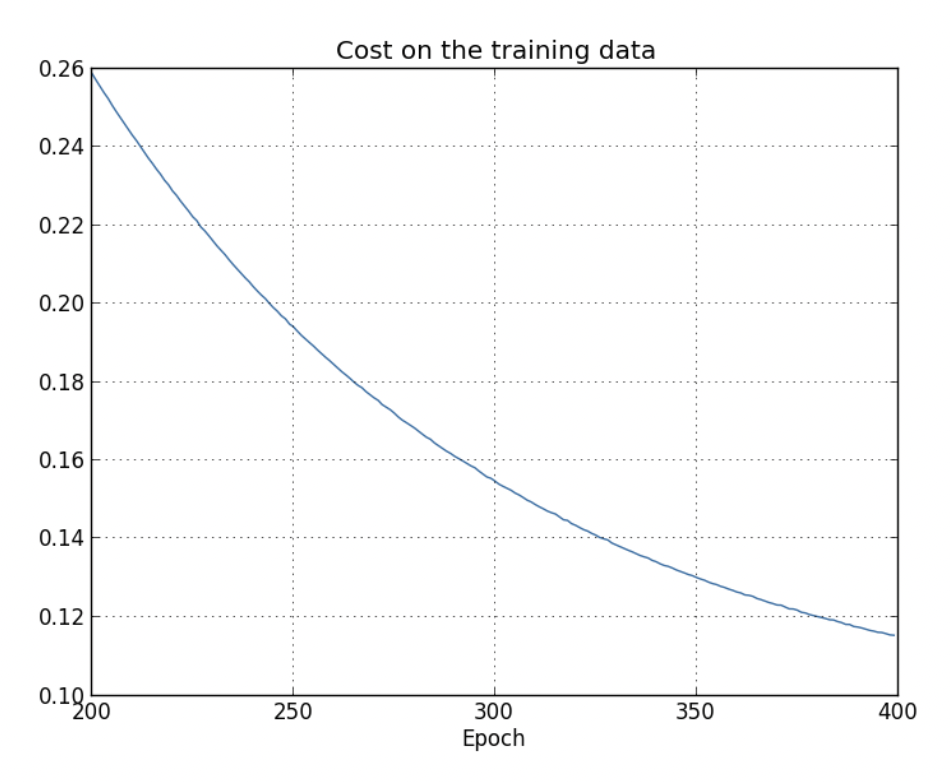
\includegraphics[scale=.29]{reg-cost}
  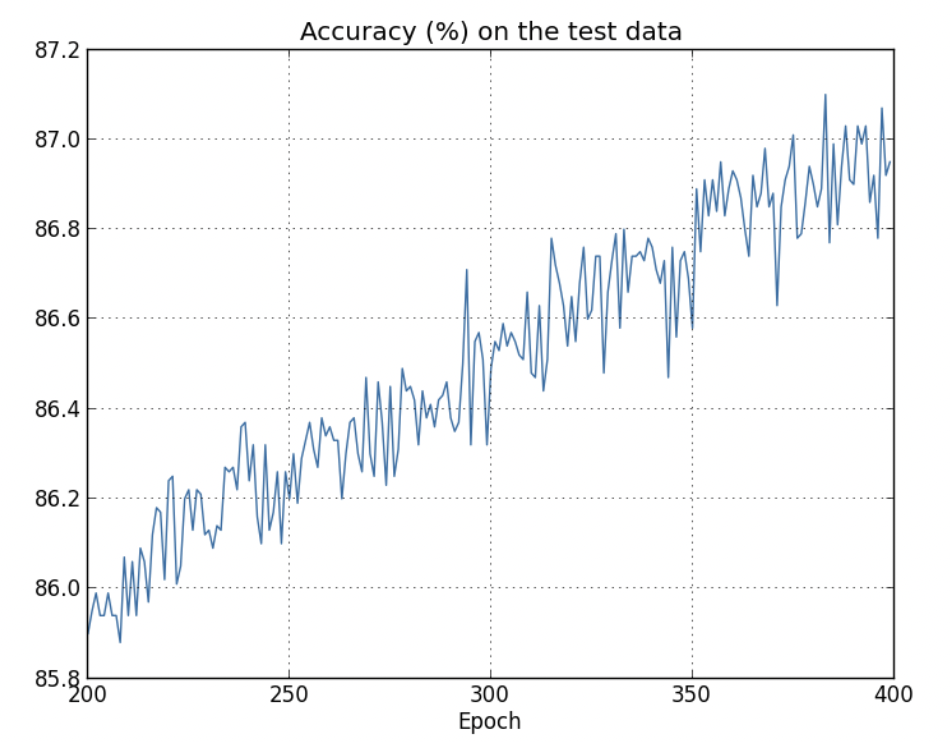
\includegraphics[scale=.29]{reg-accuracy}
  \end{center}
  \end{minipage} \hfill \pause \begin{minipage}{.4\textwidth}
  \begin{center}
  {\tiny Without regularization}
  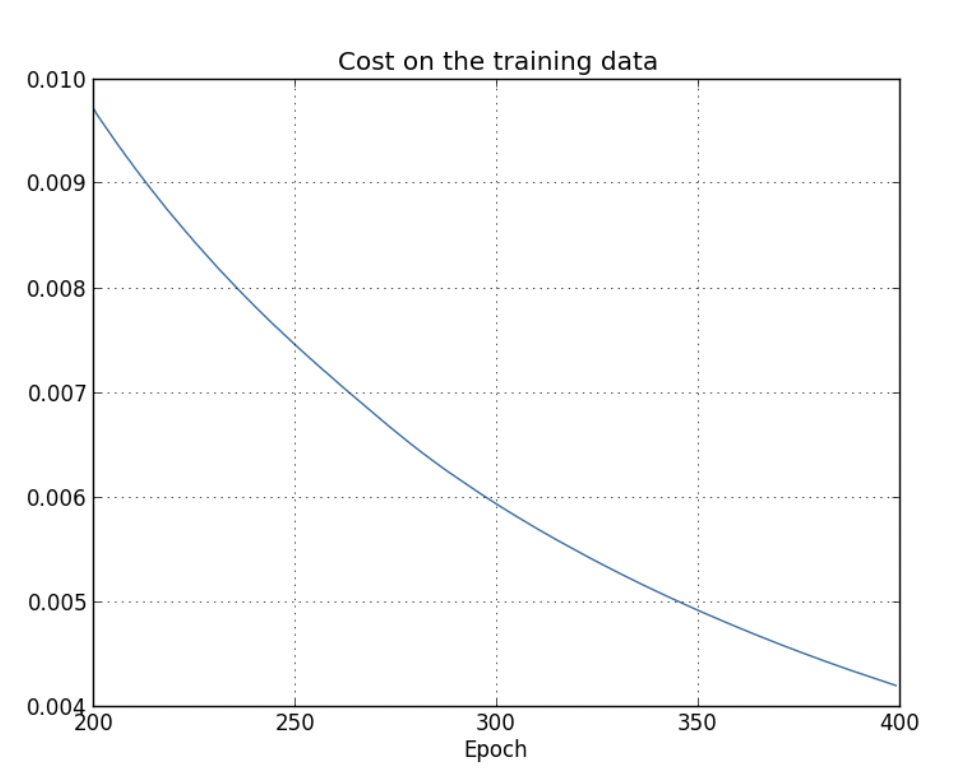
\includegraphics[scale=.29]{cost-train}
  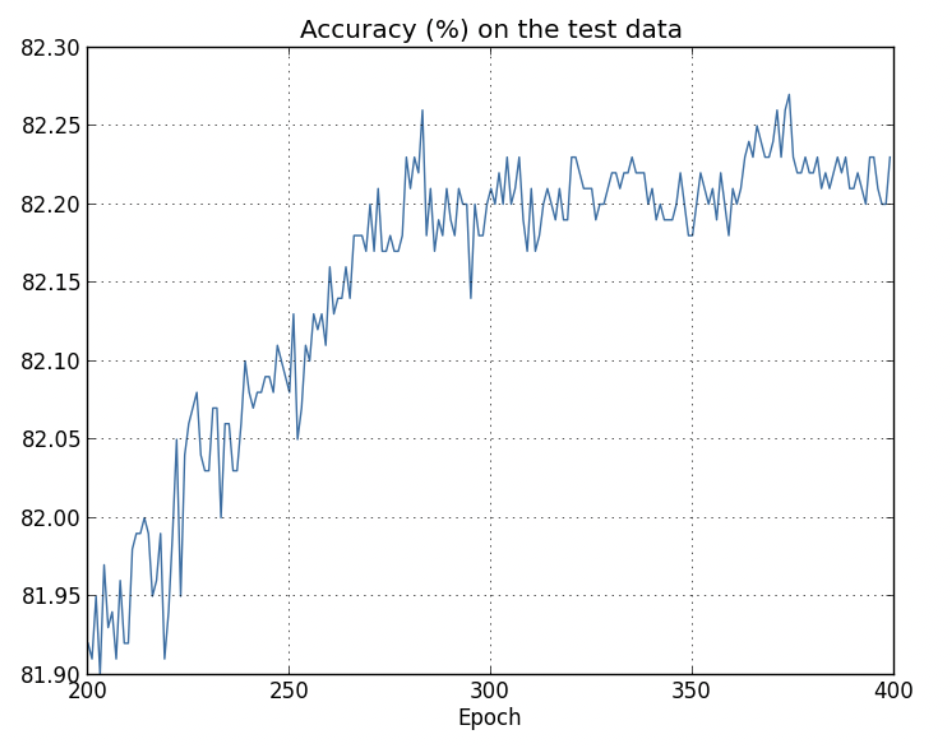
\includegraphics[scale=.29]{accuracy-test}
  \end{center}	
 \end{minipage}

\end{frame}

%%%%%%%%%%%%%%%%%%%%%%%%%%%%%%%%%%%%%%%

\begin{frame}
  \frametitle{Why does it work?}
  
  For empirical reasons (and kind of heuristic).
  
  \begin{alertblock}{}
Smaller weights $\approx$ lower complexity. Occam's razor: prefer simpler hypothesis to explain a phenomenon.
  \end{alertblock}
  
  \medskip
  
  Also: if weights are smaller, small changes on the inputs do not change much the outputs. And, they are resistant to noise in the training data.

  
\end{frame}
%%%%%%%%%%%%%%%%%%%%%%%%%%%%%%%%%%%%%%%%

%%%%%%%%%%%%%%%%%%%%%%%%%%%%%%%%%%%%%%%%

\begin{frame}
  \frametitle{Why are biases not regularized?}
  
  Again, mostly for empirical reasons, and convention.
  
 \largeskip
 
 However, having large biases:
 \begin{itemize}
  \item does not affect overfitting as much as having large weights and
  \item provides more flexibility, sometimes is desirable.
\end{itemize}

  
\end{frame}


%%%%%%%%%%%%%%%%%%%%%%%%%%%%%%%%%%%%%%%%%
%%%%%%%%%%%%%%%%%%%%%%%%%%%%%%%%%%%%%%%
\section{Choosing hyper-parameters}
\frame{
\setbeamercovered{transparent}
\tableofcontents[currentsection,
        currentsubsection,
        subsectionstyle=shaded]
}
%%%%%%%%%%%%%%%%%%%%%%%%%%%%%%%%%%%%%%%
\begin{frame}
  \frametitle{Importance of hyper-paramters}
  
  \begin{itemize}
  \item 30 hidden neurons;
  \item mini-batch size of 10;
  \item 30 epochs;
  \item $\eta=10$;
  \item $\lambda=1000$.
\end{itemize}

\medskip \pause

Accuracy on evaluation data: 10\%!
  
\end{frame}


%%%%%%%%%%%%%%%%%%%%%%%%%%%%%%%%%%%%%%%
\begin{frame}
  \frametitle{Coping with random results}
  
  How to (more or less) scientifically address the problem of setting the hyper-paramters?
  
  Strategies:
  \begin{itemize}
  \item try to get results fast: restrict the classification classes (and therefore training set);
  \item attack one hyper-parameter at a time, starting from $\eta$ and monitor the training cost. 
  \item move to $\lambda$ using the accuracy on evaluation set;
  \item use early stopping for the number of epochs.
\end{itemize}

\end{frame}

%%%%%%%%%%%%%%%%%%%%%%%%%%%%%%%%%%%%%%%
%%%%%%%%%%%%%%%%%%%%%%%%%%%%%%%%%%%%%%%




%%%%%%%%%%%%%%%%%%%%%%%%%%%%%%%%%%%%%%%




%%%%%%%%%%%%%%%%%%%%%%%%%%%%%%%%%%%%%%%



%%%%%%%%%%%%%%%%%%%%%%%%%%%%%%%%%%%%%%%




%%%%%%%%%%%%%%%%%%%%%%%%%%%%%%%%%%%%%%%

\end{document}